\documentclass[a4paper]{article}

\usepackage[utf8]{inputenc}   % LaTeX, comprends les accents !
\usepackage[T1]{fontenc}      % Police contenant les caractères français
\usepackage[french]{babel}  
\usepackage{fullpage}
\usepackage{graphicx}
\usepackage{wrapfig}
\usepackage{float}
\usepackage{blindtext}
\usepackage{algorithm2e}

\RestyleAlgo{ruled}
\graphicspath{ {./img/} }

\begin{document}
	\title{Reconnaissance de l'écriture manuscrite\\Rapport de projet}
	\author{Laurent Antoinette, Romain Campillo, Tony Nguyen\\\emph{L3 informatique}\\
	Faculté des Sciences\\
	Université de Montpellier.}
	\date{\today}
	\maketitle
	\thispagestyle{empty}
	\begin{figure}[h]
		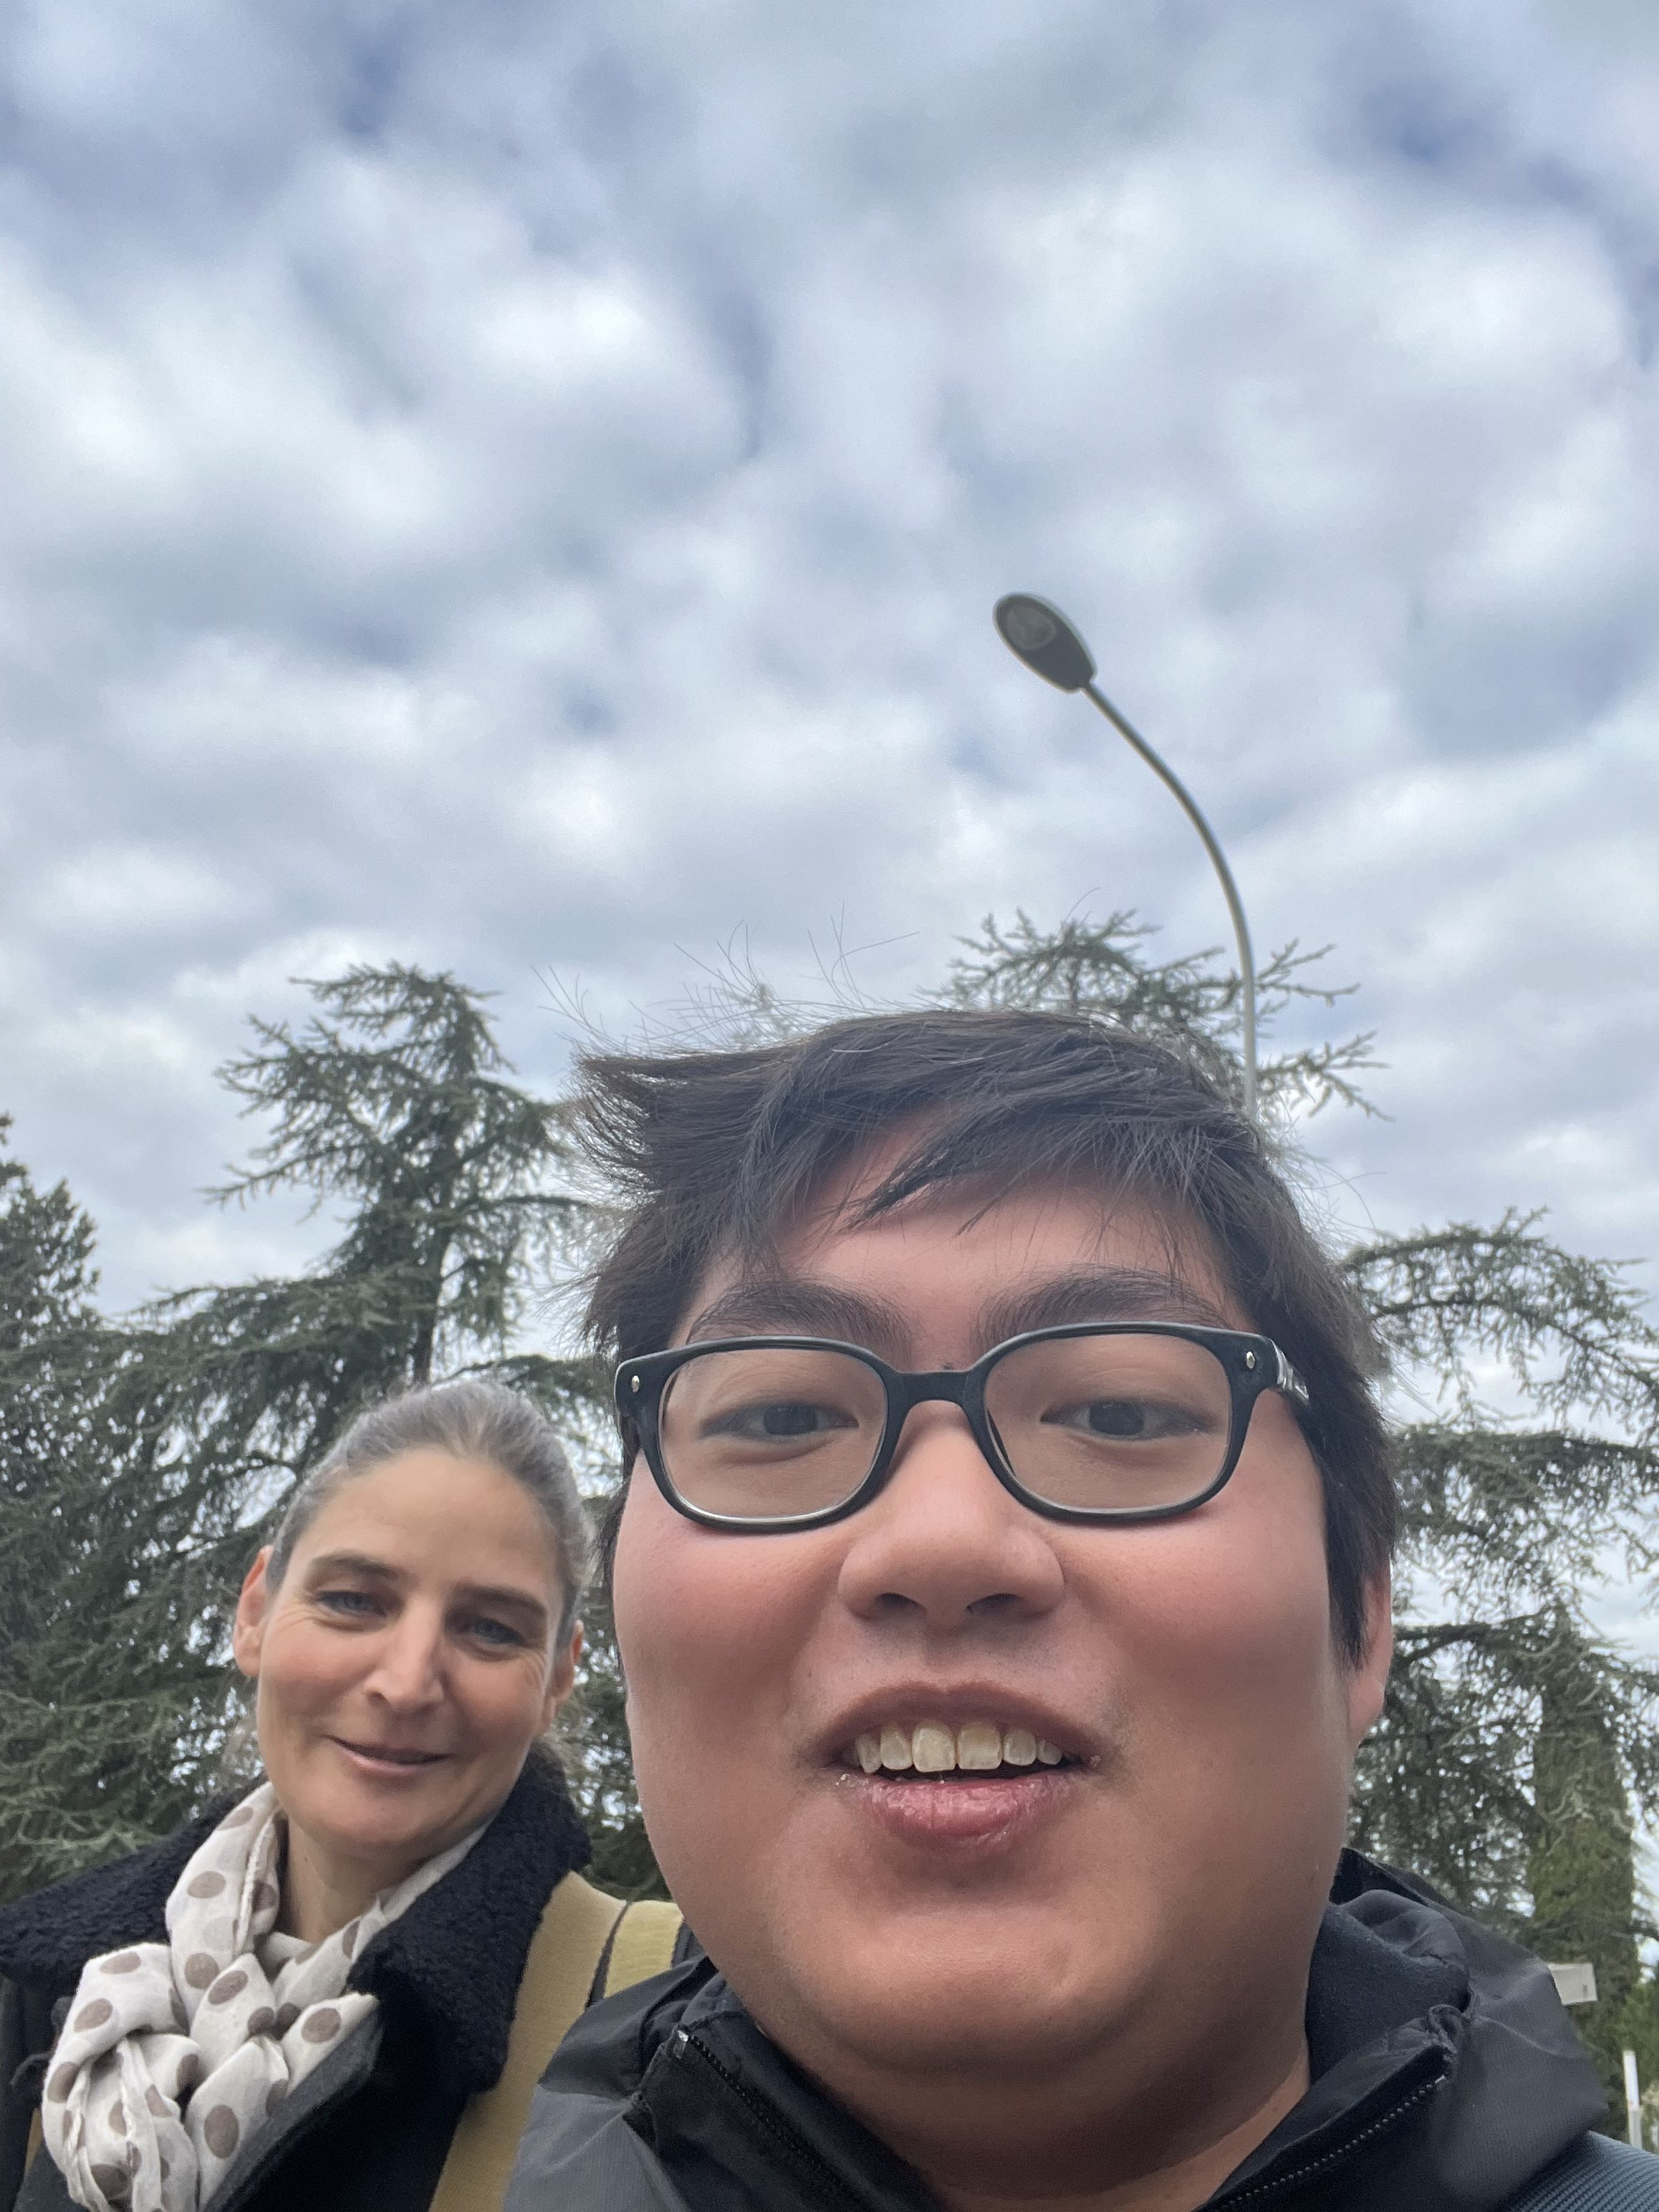
\includegraphics[scale=.1]{selfie_tony_clementine.jpg}
		% 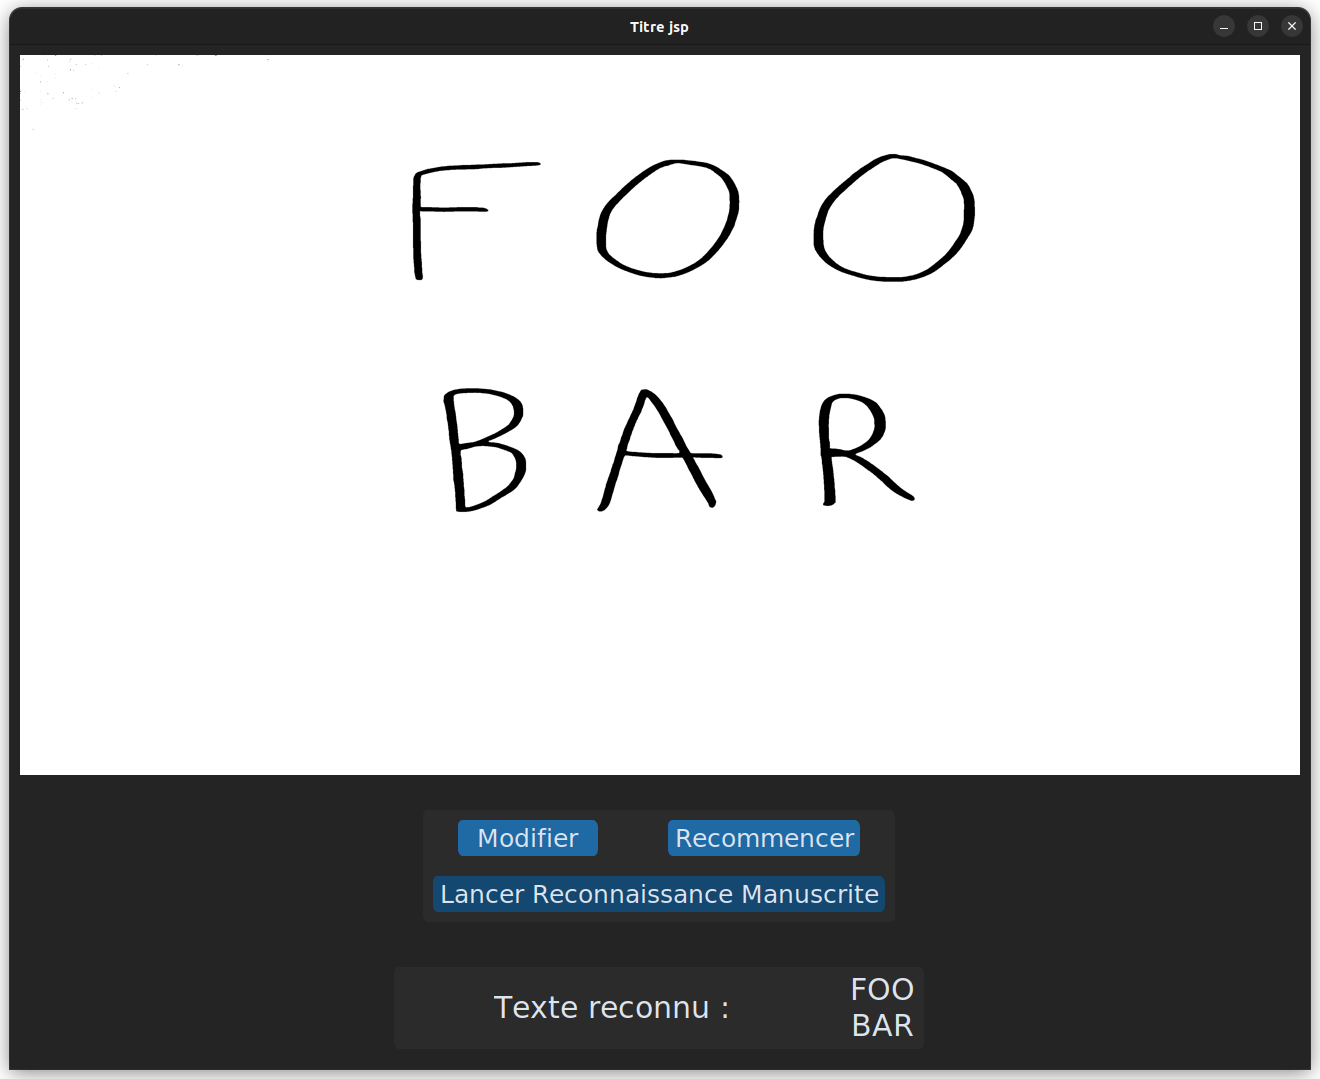
\includegraphics[width=\textwidth]{recon.png}
		\centering
	\end{figure}
	\newpage
	\thispagestyle{empty}
	\tableofcontents
	\newpage
	\thispagestyle{empty}
	\listoffigures
	\listofalgorithms
	\newpage
	\section{Présentation du Sujet } 
		\subsection{La problématique}
			L'essence du problème est qu'un texte dans un document est très diffrent d'une photo du même document. Dans le 1er cas, le format rend le contenu comprehensible par un ordinateur, il peut donc 
			chercher un mot dans le texte ou le modifier pour corriger des fautes d'orthographe. Dans le 2e cas, l'image représente la même chose. MAIS, la machine ne comprend le sens de l'information 
			représentée. Il voit les pixels mais pas les charactères. De plus, des imperfections dans la capture du document changent la photo (ex: luminosité, angle ...), il y a une modification des informations
			alors que le texte ne change pas.
			\\Réussir à lire du texte sur des images permettrait de faciliter la numérisation de document papier. Ainsi, libérer les Humains de quelques tâches redondantes. Lire des formulaires ou encore d'améliorer les moteurs de recherche avec des images qui contient du texte sont des applications possibles.
		\subsection*{}
			Ce problème est particulièrement intéressant. En effet, un projet sur le traitement automatique de l'information numérique est exactement ce que des étudiants en informatique devraient faire. Nous avons pu constater une explosion
			de l'intelligence artificielle ces dernières années. Notamment les réseaux neuronaux. À l'heure actuel, ils sont capables de detecter des objets et de les classifier. Ce projet est tout à fait 
			intéressant pour de futurs étudiants en master IASD.
		\subsection{Les différentes approches}
			\subsubsection{k-Nearest Neighbor}
				Méthode statistique, il y a un plan avec plein d'objets qui forment des troupeaux, notre lettre est quelque part dans le plan, on trace un cercle autour, notre lettre est identifiée comme l'objet présent au plus grand nombre à l'intérieur du cercle.
			\subsubsection{Template matching} 
				En gros, comparaison de l'image avec la base de donnée entière à l'aide d'une fonction de distance. 
		\subsection{Objectifs}
			Notre but est de créer un logiciel pour tranformer une image qui contient des symboles en un texte numérique.\\
			Initialement, nous nous concentrerons sur des images simples et de bonne qualité avec des symboles de l'alphabet latin (26 lettres) seulement en majuscules sur 1 ligne. Puis, si le temps nous le permet, on aggrandira la portée du problème.
		\subsection{Cahier des charges}
			\subsubsection{Besoins et contraintes}
				\paragraph{Les besoins}
					\subparagraph{Capturer une image}
						L'utilisateur pourra prendre des photos par notre logiciel à l'aide d'une webcam. Mais il pourra également utiliser des images depuis son système de fichier. Tout cela à travers une interface Homme-Machine.
					\subparagraph{Pré-traitement}
						Le logiciel réduira le bruit et rendra l'image plus nette à l'aide de plusieurs filtres prédéfinis. 
					\subparagraph{Segmentation de l'image}
						Les différents charactères présents sur l'image seront localisés à l'aide d'histogramme de projection.
					\subparagraph{Extraction des charactères}
						Les charactères seront ensuite découpés pour former leurs propres imagettes .i.e une image qui contient TEST devriendra 4 petites imagettes contenant respectivement T E S T.
					\subparagraph{Reconnaissance}
						Les imagettes feront l'objet d'une reconnaissance de façon individuelle. La solution que nous choisissons d'implémenter est un réseau neuronal convolutif.
					\subparagraph{Présenter}
						Une fois que les imagettes sont reconnues en charactère. Il est nécessaire de les assembler et d'afficher à l'utilisateur les mots reconnus.
				\paragraph{Les contraintes}
					Nous nous fixons comme contraintes de ne pas utiliser de services comme Google Collab car Google possède un modèle économique type "Freemium" (initialement gratuit mais avec des fonctinalités payantes). Nous souhaitons créer un logiciel suffisament performant pour qu'il puisse être lancé sur l'une de nos machines personelles. \\De plus, une webcam est nécessaire, ou alors un appareil photo numérique.
			\subsubsection{Résulats attendus}
				\paragraph{}
					Notre programme doit reconnaître des lettres manuscrites sur un fond blanc. Les lettres seront des charactères majuscule non-liées et sans accents ni charactère spécial.
	\section{Technologies utilisées} 
		\subsection{Langages et outils}
			\subsubsection{Python3}
			\subsubsection{OpenCV}
				\begin{wrapfigure}{r}{0.15\textwidth}
					
\includegraphics[width=0.15\textwidth]{OpenCV.png}
				\end{wrapfigure}
				Dans ce projet, nous choisissons d'utiliser la librairie open source de vision par ordinateur (Open Computer Vision). Elle contient les fonctionnalités de pré-traitement d'image nécessaire dans ce projet. Nous utiliserons surtout les fonctions de filtrage d'image.
				\newline
			\subsubsection{You Only Look Once}
				You Only Look Once (YOLO) est une archicture de Réseau Neuronal Convolutif (CNN) de type "Region based" (R-CNN) qui est capable de localiser des objets dans une image et en même temps, les classifier.
				\paragraph{Expliquons (un peu tout petit peu) plus en détail les réseaux neuronaux}
					Les réseaux de neurone simulent plus ou moins le fonctionnement de notre cerveau. Parlons d'abord de l'élément le plus petit et on va progresser jusqu'aux CNN.
					\subparagraph{Le neurone} va prendre plusieurs entrées, des nombres, faire une opération avec une fonction d'activation et en sortie retourner le résultat.
					\subparagraph{Réseau de neurone} L'architecture des réseaux de neurone simple est organisée en couche. La 1er couche qui est l'entrée (censée reprensenter les yeux).
						La dernière couche représente la sortie, par exemple si le réseau est entrainé pour reconnaitre des chiens, la sortie doit retourner une valeur proche de 1 si c'est un chien et 0 sinon.
						Entre le début et la fin du réseau, les couches intermédiaires sont connectées vers l'avant et de façon complète. Un neurone est connecté à tous les neurones de la couche précédente et suivante mais pas à ceux de la même couche.
					\\Le désavantages de cette approche est qu'il est nécessaire de lui donner des "charactéristiques". Pour reconnaitre si cet animal est un chien on ne va pas lui donner l'image directement, on va lui dire en entrée si ça a des poils, la couleur de son pelage, le nombre de pattes, la forme des oreilles.
					\subparagraph{Les CNN} blablabla
					\subparagraph{R-CNN}
		\subsection*{test}
			\blindtext
	\newpage
	\section{Développements Logiciel : Conception, Modélisation, Implémentation}
		\begin{figure}[h]
			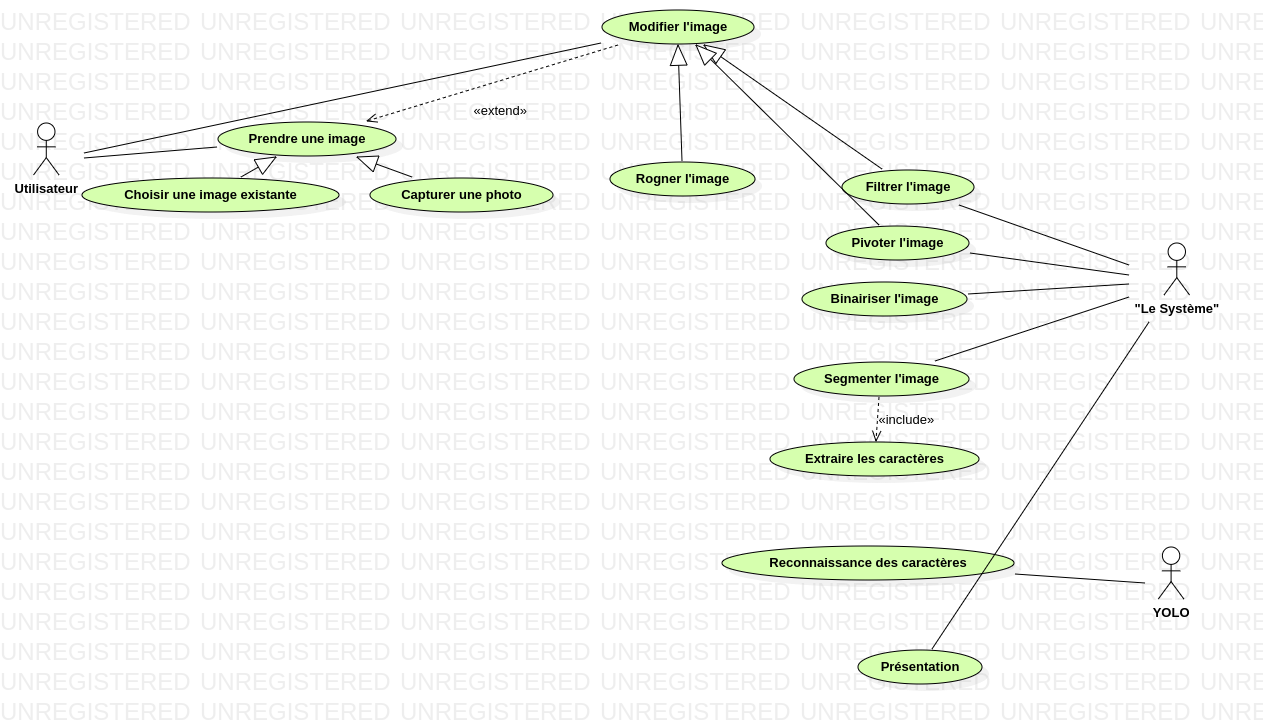
\includegraphics[width=\textwidth]{UseCaseDiagram.png}
			\centering
			\caption{Diagramme de cas d'utilisation}
			\label{fig:useCaseDiagram}
		\end{figure}
		\subsection{Interface Homme-Machine}
			L'IHM nous permet de prendre des photos avec une webcam connectée à l'ordinateur ou choisir à partir d'une fenêtre une image déjà existante. 
%Diagramme de Cas d'Utilisation à la page \pageref{fig:useCaseDiagram}. 
			\begin{figure}[H]
				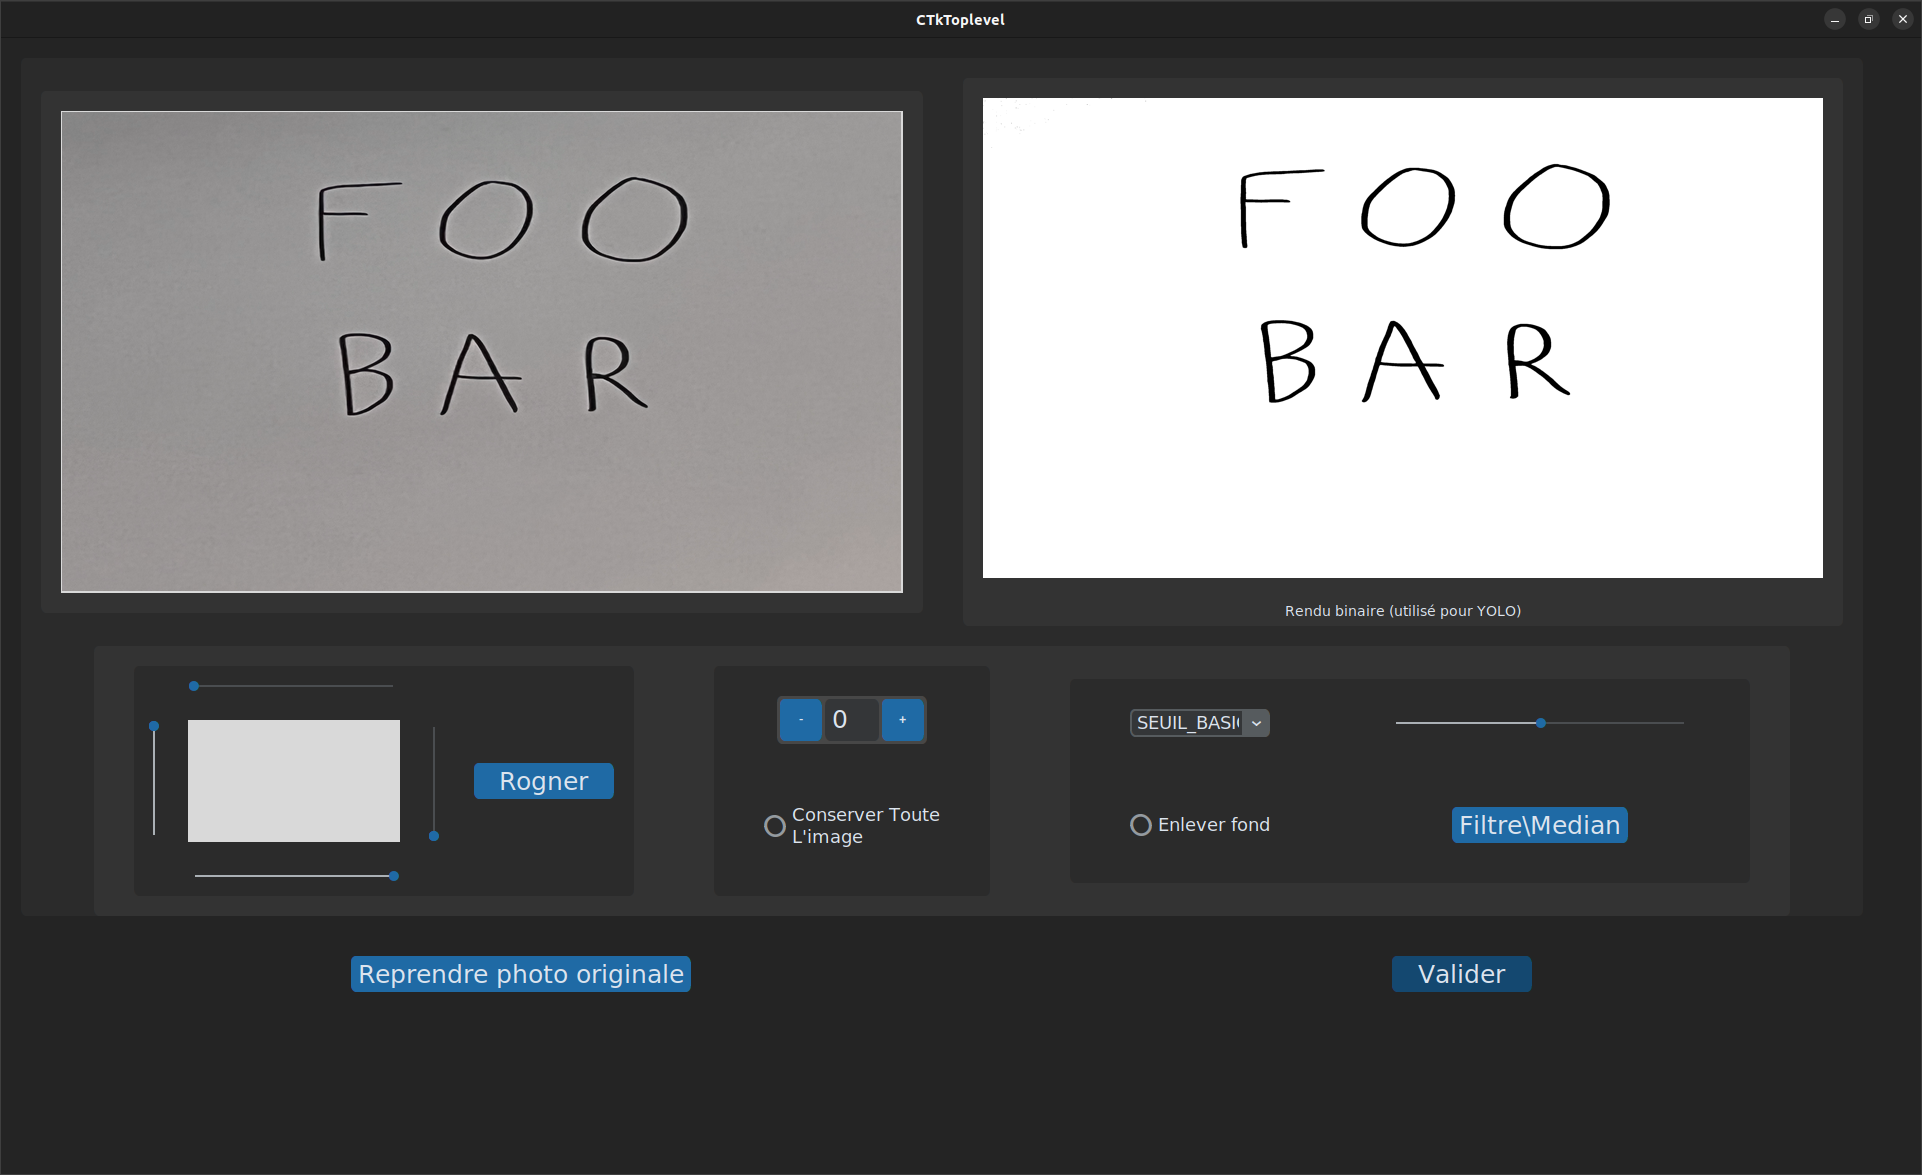
\includegraphics[width=0.8\textwidth]{modif.png}
				\centering
				\caption{Fenêtre de l'IHM où l'on peut rogner, pivoter et filtrer une image}
				\label{fig:modif}
			\end{figure}
			\paragraph{}
				Après avoir entrer une image, il est possible qu'il y ait beaucoup de bruit, dans ce cas là, nous pouvons rogner l'image pour enlever des ombres sur les bords, faire des rotations et filtrer pour enlever le bruit comme illustrée sur la figure \ref{fig:modif}
			\begin{figure}[H]
				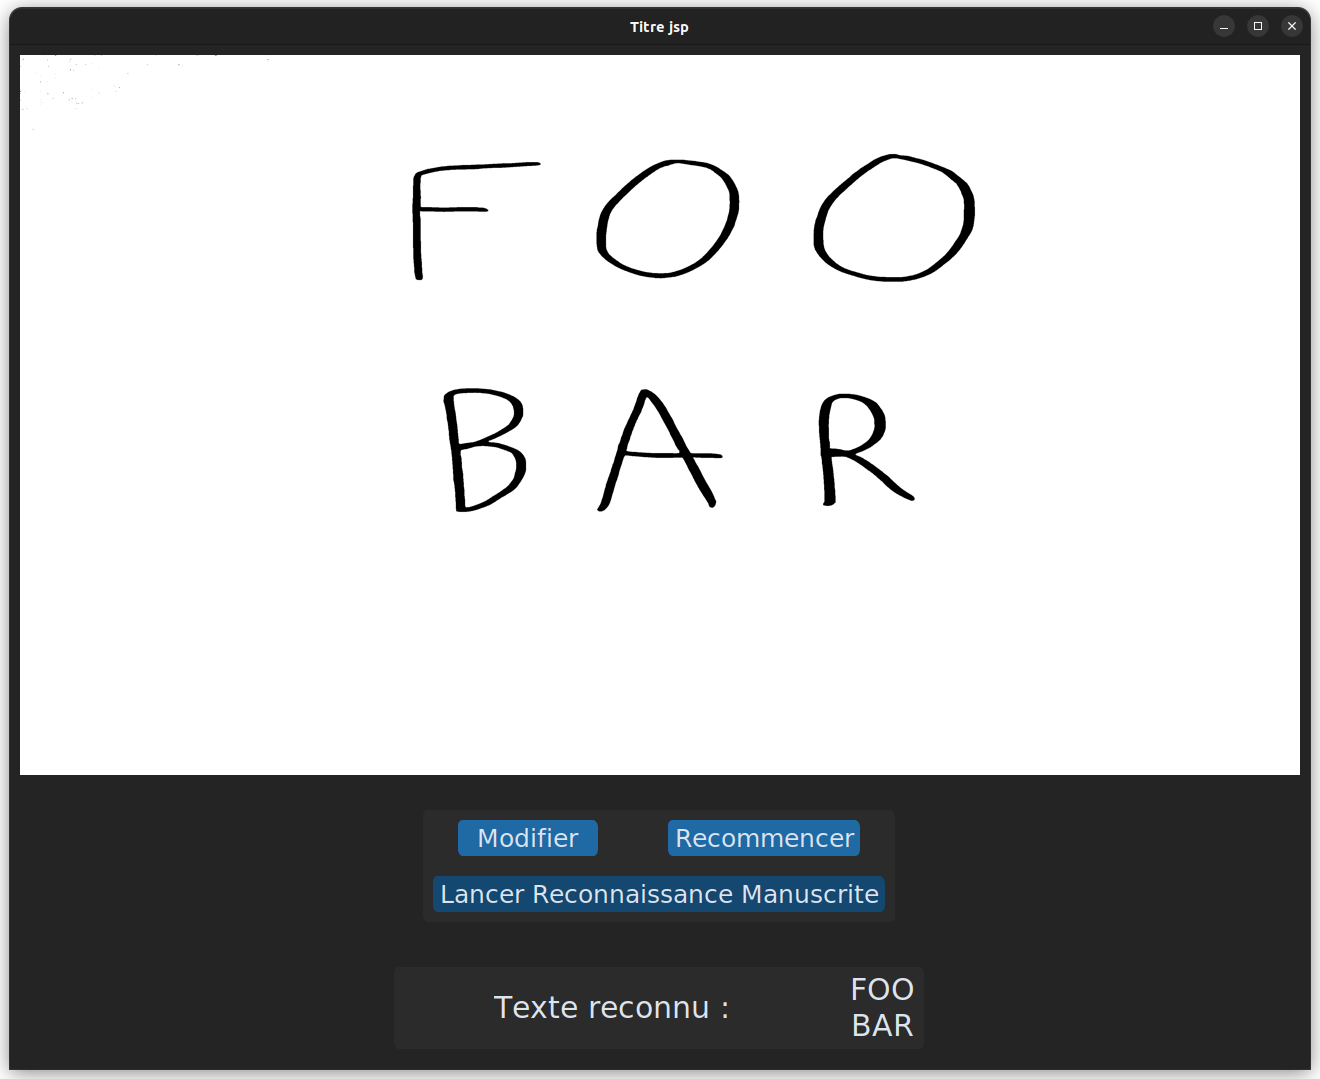
\includegraphics[width=0.8\textwidth]{recon.png}
				\centering
				\caption{Fenêtre de l'IHM après présentation des charactères reconnus}
				\label{fig:recon}
			\end{figure}
			\paragraph{}Sur la figure \ref{fig:recon}, on peut voir qu'après avoir obtenu une image de bonne qualité, notre programme va segmenter les charactères, en faire des imagettes et donner ces imagettes individuellement à YOLO. Ensuite après cette reconnaissance, l'IHM présente le résultat.
			\paragraph{}Il est possible de voir les imagettes générées dans le dossier "./images/imageSegmentee"
		\subsection{Procédures de lecture et validation des entrées}
			beep	
		\subsection{Statistiques}
			\begin{itemize}
				\item[•] Nombres de lignes de code : 
				\item[•] Nombres de script
			\end{itemize}
	\section{Algorithmes et Analyse}
		\subsection{YOLO}
		\subsection{Segmentation par histogramme de projection}
			\begin{algorithm}
				\SetKwInput{Strat}{Stratégie}
				\LinesNumbered
				\caption{SEGMENTATION(image)}\label{alg:segmentation}
				\KwData{image en RGB}
				% \KwOut{output}
				% \KwOut{output}
				\Strat{D'abord, une segmentation des lignes par projection vertical. 
				Puis, dans un 2e temps, segmentation des caractères grâce à une projection horizontal de chaque ligne individuellement}
				\KwResult{\\Tableau de couples d'entier représentant les coordonnées y de début et de fin des lignes sur l'image
        				\\Tableau de tableau de couple d'entier représentant les coordonnée x de début et de fin des lettres par lignes, 
        				\\Tableau d'image des lignes
        				\\Tableau de tableau d'image des caractères}
				\BlankLine
				$ndgImage \gets convertirImageEnNDG(image)$\;
				\BlankLine
				\tcc{on met l'image en noir et blanc sauf que le seuillage est inversé}
				$imageBinaire \gets binarisationInversé(ndgImage)$\;
				\BlankLine
				\tcc{on fait la somme des pixels sur les colomnes et on les divise par 255}
				$projectionHorizontale = (sommeValPixel(imageBinaire, axe=1)) / 255$\;
				$delimitationDesLignes = coordonneeLigne(projectionHorizontal)$\;
				\BlankLine
				$imagesLignes = []$\;
				\BlankLine
				\tcc{on copie une zone de l'image correspondant à un caractère grâce aux coordonnées calculées\\et on l'ajoute à notre tableau d'image des lignes}
				\For{(x,y) dans delimitationDesLignes}{imagesLignes.ajouter(ndgImage[x:y, 0:longeurImage])}
				\BlankLine
				\tcc{on initialise le tableau de tableaux des images de Caractère on fonction du nombre de ligne detecté}
				$imagesCaracteres = [[ ] pour i allant de 0 à longeur(imagesLignes)]$\;
				\BlankLine
				\tcc{on initialise le tableau de tableaux de couple de coordonnées  on fonction du nombre de ligne}
				$coordonneesCaracteres = [[] pour i allant de 0 à longeur(imagesLignes)]$\;
				\BlankLine
				\For(){index, uneLigne dans imagesLignes}
				{
					$ligneBinaire = binarisationInversé(uneLigne)$\;
					\tcc{on fait la somme des pixels sur les lignes et on les divise par 255}
					$projectionVerticale = (sommeValPixel(imageBinaire, axe=0)) / 255$\;
					$delimitationDesCaracteres = coordonneeCaractere(projectionVerticale)$\;
					\BlankLine
					\tcc{on ajoute les coordonnées au tableau de coordonnées}
					$coordonneeCaractere[index].ajouter(delimitationDesCaracteres)$\;
					\tcc{on copie une zone de l'image correspondant à un caractère grâce aux coordonnées calculées\\et on l'ajoute à notre tableau d'image de caractère}
    				\For(){(x,y) dans delimitationDesCaracteres}
					{
						$imagesCaracteres[index].ajouter(ndgImage[0:hauteurUneLigne, x:y])$\;
					}
					$redimensionnerImage(imagesCaracteres[index],hauteur = 128,longeur = 128)$\;
					\BlankLine
				}
				\KwRet{$delimitationDesLignes,delimitationDesCaracteres,imagesLignes,imagesCaracteres$}
			\end{algorithm}
			\newpage
			\begin{algorithm}
				\SetKwInput{Strat}{Stratégie}
				\LinesNumbered
				\caption{COORDONNEECARACTERE(T)}\label{alg:coordcar}
				\KwData{tableau de flottant représentant la projection vertical d'une image}
				\Strat{Trouver les zones non nul dans l'histogramme}
				\KwResult{tableau de couple d'entier indiquant les coordonnées du début et de la fin d'une lettre}
				\BlankLine
				$coordCaractere = []$\;
				\BlankLine
				$dansLeCaractere = False$\;
				\tcc{Début = pair	Fin = impair}
				$DF = []$\;
				\BlankLine
				\For{i de 0 à taille(T)}
				{
					\If{$T[i] \neq 0$}{
						\If{!dansLeCaractere \textbf{or} (dansLeCaractere  \textbf{and} i == taille(T)-1)} {
							$DF.ajouter(i)$\;
						}
						$dansLeCaractere = True$\;
					}
					\Else{
						\If{dansLeCaractere} {
							DF.ajouter(i)
						}
						$dansLeCaractere = False$\;
					}
				}
				$lettres = [ (DF[i],DF[i+1]) pour i de 0 à taille(DF) avec un pas de 2 ]$\;
				\BlankLine
				$tailleEspacesEntrelettres = [ lettres[i+1][0]-lettres[i][1] pour i de 0 à taille(lettres)-1 ]$\;
				$poidsEspace = trillageCroissant(tailleEspacesEntrelettres)$\;
				\BlankLine
				$SommeIndice \gets 0$\;
				\For{i de 0 à taille(poidsEspace)-1}
				{
					$poidsEspace[i] \gets poidsEspace[i] * (taille(poidsEspace)-i)$\;
				    $SI \gets SI + i$\;
				}
				$moyenneEspaces \gets somme(poidsEspace) / SI$\;
				$j \gets 0$\;
				\While{tailleEspacesEntrelettres != []}
				{
					\If{$tailleEspacesEntrelettres < moyenneEspaces*0.2$} {
						$D = lettres[j];$ $supprimer(lettres[j])$\;
						$F = lettres[j];$ $supprimer(lettres[j]);$\;
						\tcc{inserer(tableau, indice, élément)}
						$inserer(lettres,j,(D[0],F[1]))$\;
					}	\lElse{$j \gets j+1$}
					$supprimer(tailleEspacesEntrelettres[0])$\;
				}
				\KwRet{lettres}
			\end{algorithm}
			\begin{figure}
				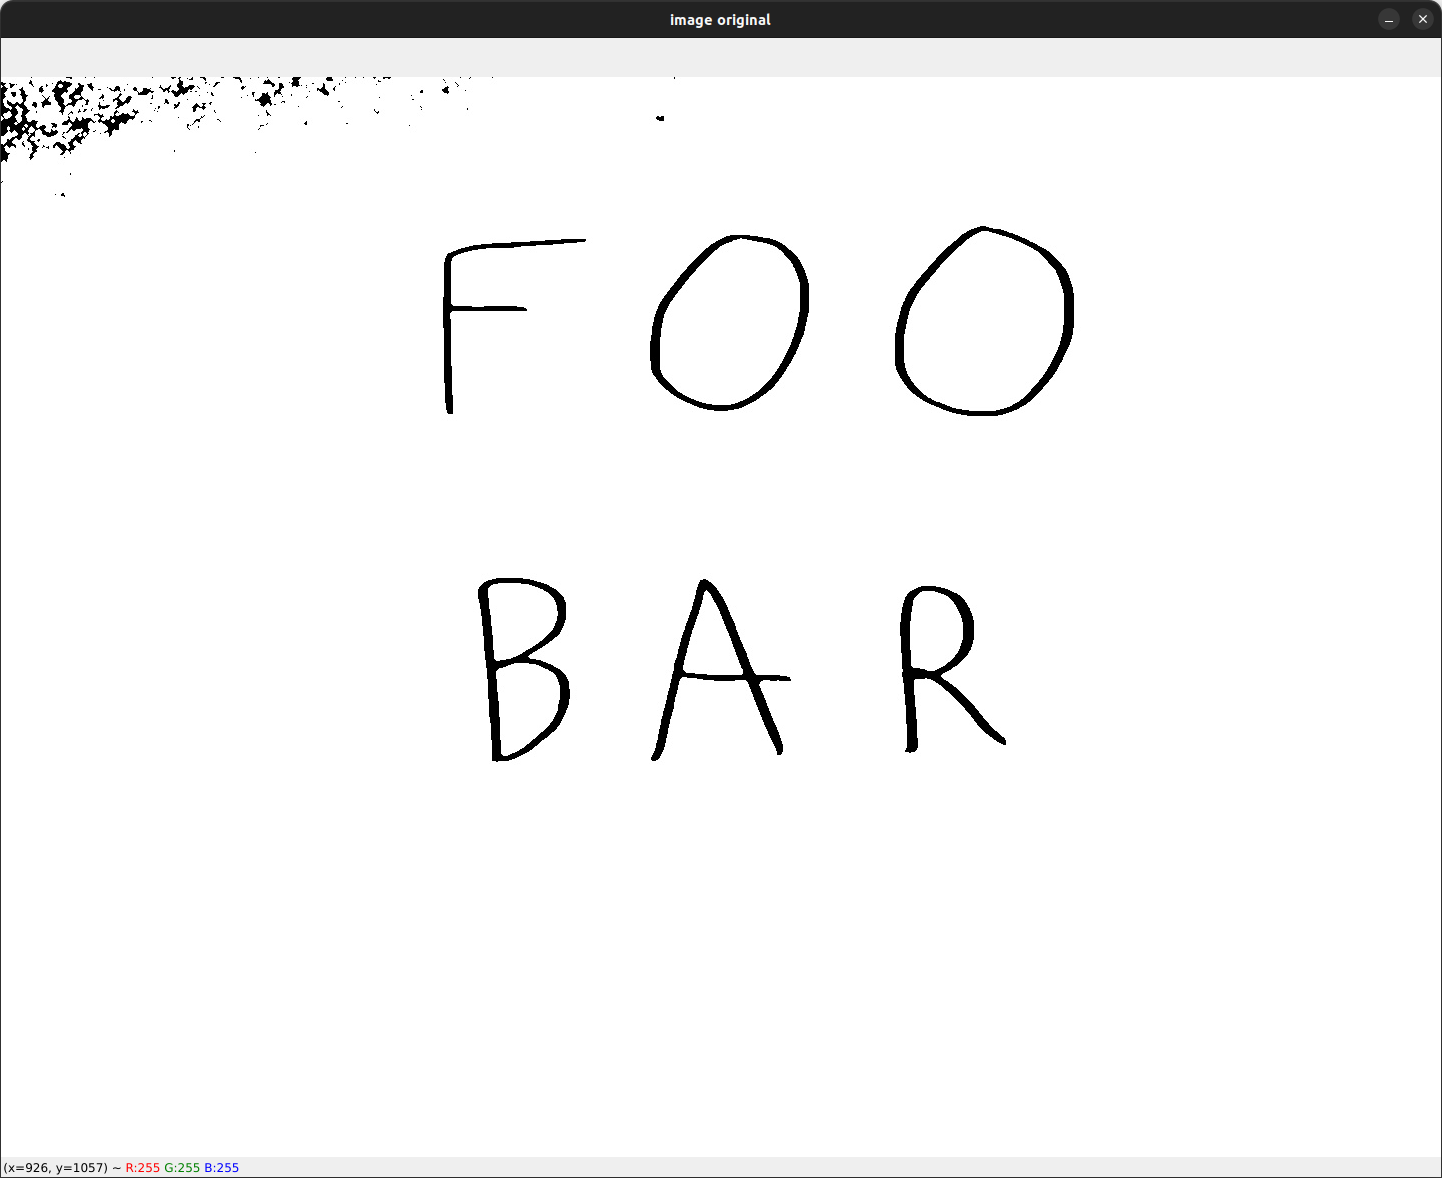
\includegraphics[width=\textwidth]{segmentation_image_originel.png}
				\centering
				\caption{Exemple d'une image après filtrage}
				\label{fig:imageOriginel}
			\end{figure}
			\paragraph{} Sur la figure \ref{fig:imageOriginel}, nous voyons une image de bonne qualité prête à être segmenter par l'algorithme n°\ref{alg:segmentation} (page \pageref{alg:segmentation}). 
			\begin{figure}
				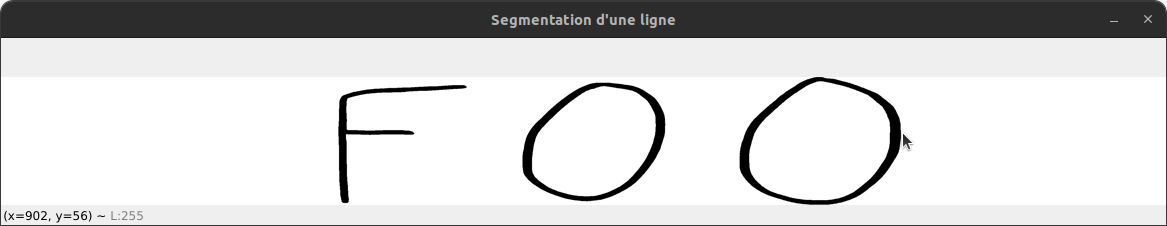
\includegraphics[width=.8\textwidth]{segmentation_ligne1.png}
				\centering
				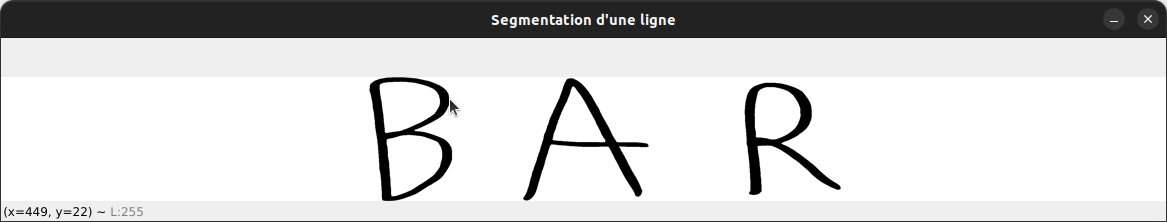
\includegraphics[width=.8\textwidth]{segmentation_ligne2.png}
				\centering
				\caption{Images de nos 3 lignes crée à partir de l'image de départ}
				\label{fig:imageLignes}
			\end{figure}
			% \paragraph{} On voit sur la figure \ref{fig:imageLignes} à la page \pageref{fig:imageLignes} que dû à un filtrage de bonne qualité, nous obtenons exactement 2 lignes comme attendus. 
			\begin{wrapfigure}{r}{0.35\textwidth}
					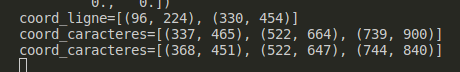
\includegraphics[width=0.35\textwidth]{structDonnee.png}
					\caption{Structure de données dans l'algorithme SEGMENTATION}
					\label{fig:structDonnee}
			\end{wrapfigure}
			\paragraph{} Grâce à une projection vertical, nous obtenons ce tableau (voir figure \ref{fig:structDonnee}). La 1er ligne de ce tableau contient autant de tuples que le nombre de lignes. Chaque tuples contient la commposante en ordonnée du début et de la fin d'une ligne. En choississant arbitrairement comme largeur d'une ligne, la largeur de l'image, on extrait nos 2 lignes comme sur la figure \ref{fig:imageLignes}.
			\paragraph{} Maintenant que nous avons isoler les lignes, nous allons maintenant découper les lettres de chaque lignes en suivant l'algorithme n°\ref{alg:coordcar} page \pageref{alg:coordcar}
			\paragraph{} Étant donnée que l'image est filtré, en noir et blanc et binairisé, lorsqu'une lettre est présente à un endroit donnée, cela signifie que sur la projection vertical, l'histogramme est supérieur à 0 à cet endroit là. Sinon, il n'y a pas de lettre et l'histogramme est à 0. L'algorithme n°\ref{alg:coordcar} va parcourir totalement l'histogramme de projection et va tenté de dectecter ces "zones pleines" et récupérer l'indice de début et de fin de ces zones qui correspondront à la limite gauche et droit de la lettre sur l'image. Nous pouvons voir le résultats de cette fonction sur la figure \ref{fig:structDonnee} et il y a extrait d'un histogramme horizontal dans l'annexe (page \pageref{fig:histoX}).
			\begin{figure}
				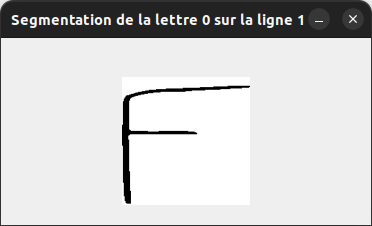
\includegraphics[scale=.3]{segmentation_F.png}
				\centering
				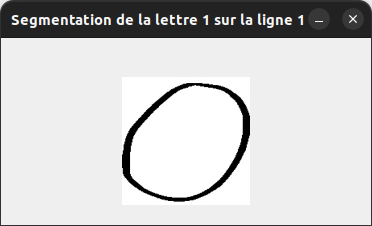
\includegraphics[scale=.3]{segmentation_O1.png}
				\centering
				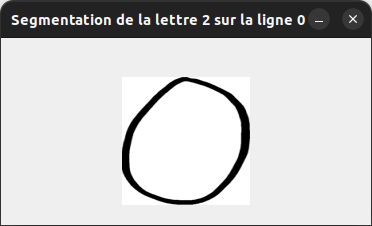
\includegraphics[scale=.3]{segmentation_O2.png}
				\centering
				\caption{Imagettes des charactères crée à partir de la 1e ligne}
			\end{figure}
			\begin{figure}
				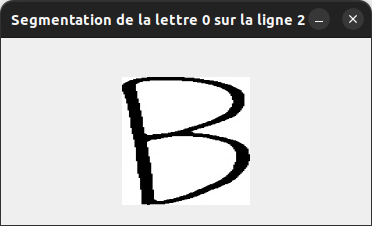
\includegraphics[scale=.3]{segmentation_B.png}
				\centering
				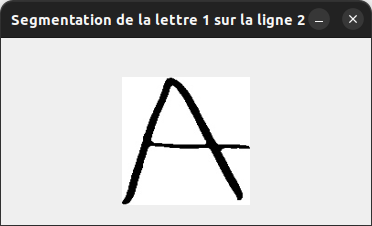
\includegraphics[scale=.3]{segmentation_A.png}
				\centering
				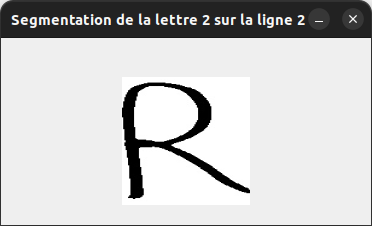
\includegraphics[scale=.3]{segmentation_R.png}
				\centering
				\caption{Imagettes des charactères crée à partir de la 2e ligne}
			\end{figure}
	\newpage
	\section{Analyse des Résulats}
		TBD
	\section{Gestion du Projet}
		\paragraph{} Pendant ce projet, nous avons due communiquer et collaborer ensembles afin d'atteindre not but commun. Voici les outils que nous avons utilisé.
		\paragraph{} Premierement, pour communiquer nous avons utiliser l'application Discord. Sur lequel nous avons un groupe où nous nous envoyons des messages, des images et des fichiers.
		\paragraph{} Ensuite, pour le partage et le versioning, nous utilisons git et Github
		Laurent : filtrage, segmentation
		Romain : IHM, YOLO
		Tony : rapport
	\addcontentsline{toc}{section}{Bilan et Conclusions}%insert dans le toc
	\section*{Bilan et Conclusions}%sans numéro et pas dans le toc
		\paragraph{}
			tests
		\paragraph{}
			Cependant, certains points laissent à désirer dans notre projet. Malheureusement, une contribution de l'utilisateur est nécessaire. Pour une bonne reconnaissance des charactères, l'utilisateur doit rogner l'image. Il serait plus pratique que le \emph{rognagne soit fait automatiquement}. 
		\paragraph{}
			Ensuite, au niveau de la \emph{segmentation}, notre algorithme n'est pas capable de séparer des lettre cursives et ignore totalement les espaces.
		\paragraph{}
			Et enfin, dans le futur, le but sera que \emph{YOLO} reconnaisse aussi l'alphabet minuscule mais aussi l'alphabet français (avec les accents).
%		meilleur segmentation : segmentation des lettres cursives, reconnaissance des espaces
%		modifier les hyper paramètres de yolo
%		YOLO : lettres minuscule, avec accents
	\newpage
	\section*{Bibliographie}
		TBD
	\section*{Annexes}
		\begin{figure}
				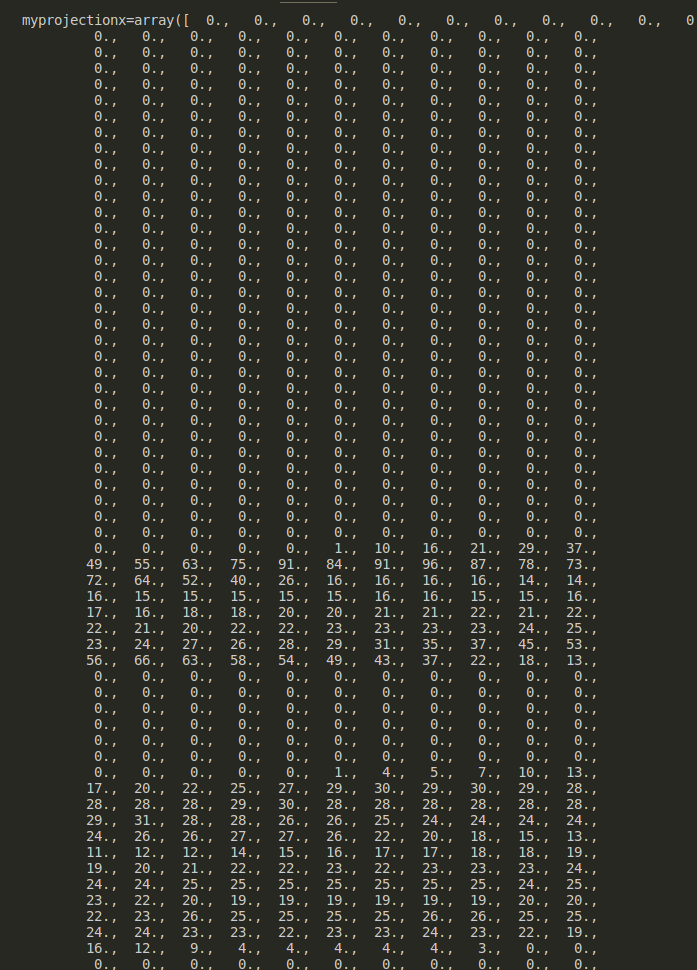
\includegraphics[width=\textwidth]{histoX.png}
				\centering
				\caption{Extrait d'un histogramme de projection horizontal}
				\label{fig:histoX}
			\end{figure}
\end{document}